\subsection{两个平面平行的判定和性质}\label{subsec:1-13}

判定两个平面平行,除根据定义外,有下面的定理:

\begin{dingli}[两个平面平行的判定定理][dl:lgpmpx-pd]
    如果一个平面内有两条相交直线都平行于另一个平面,那么这两个平面平行。
\end{dingli}

已知:在平面 $\beta$ 内,有两条相交直线 $a$、$b$ 和平面 $\alpha$ 平行(图 \ref{fig:ltjh-1-39})。

\begin{wrapfigure}[8]{r}{7cm}
    \centering
    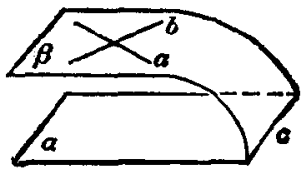
\includegraphics[width=5cm]{../pic/ltjh-ch1-39.png}
    \caption{}\label{fig:ltjh-1-39}
\end{wrapfigure}

求证:$\beta \pingxing \alpha$。

证明:假设 $\alpha \cap \beta = c$。

$\because$ \quad $a \pingxing \alpha$, $a \subset \beta$,

$\therefore$ \quad $a \pingxing c$。

同理 \quad $b \pingxing c$。

$\therefore$ \quad $a \pingxing b$。

这与题设 $a$ 与 $b$ 是相交直线矛盾,

$\therefore$ \quad $\alpha \pingxing \beta$。

在判断一个平面是否水平时,把水准器在这个平面上交叉地放两次,如果水准器的气泡都是居中的,
就可以判定这个平面和水平面平行,它的根据就是这个判定定理。


\liti \zhongdian{垂直于同一条直线的两个平面平行。}

已知:$\alpha \perp AA'$, $\beta \perp AA'$(图 \ref{fig:ltjh-1-40})。

求证: $\alpha \pingxing \beta$。

\zhengming 设经过直线 $AA'$ 的两个平面 $\gamma$、$\delta$ 分别与平面 $\alpha$、$\beta$
交于直线 $a$、$a'$ 和 $b$、$b'$。

$\because$ \quad $AA' \perp \alpha$, $AA' \perp \beta$,

$\therefore$ \quad $AA' \perp a$, $AA' \perp a'$。

$\therefore$ \quad $a \pingxing a'$。

则\quad $a' \pingxing \alpha$。

同理,$b' \pingxing \alpha$。

\hspace*{-1.5em} 又 $\because$ \quad $a' \cap b' = A'$,

$\therefore$ \quad $\alpha \pingxing \beta$。

\begin{figure}[htbp]
    \centering
    \begin{minipage}[b]{7cm}
        \centering
        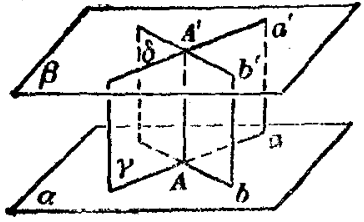
\includegraphics[width=6cm]{../pic/ltjh-ch1-40.png}
        \caption{}\label{fig:ltjh-1-40}
    \end{minipage}
    \qquad
    \begin{minipage}[b]{7cm}
        \centering
        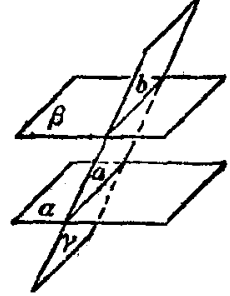
\includegraphics[width=4cm]{../pic/ltjh-ch1-41.png}
        \caption{}\label{fig:ltjh-1-41}
    \end{minipage}
\end{figure}

下面研究两个平面平行的性质。

根据两个平面平行及直线和平面平行的定义可知,
\zhongdian{两个平面平行,其中一个平面内的直线必平行于另一个平面。}

如果两个平行平面 $\alpha$、$\beta$ 与另一个平面 $\gamma$ 相交,
现在我们来研究两条交线 $a$、$b$ 的位置关系(图 \ref{fig:ltjh-1-41})。

因为 $\alpha \pingxing \beta$, 所以平面 $\alpha$ 与 $\beta$ 没有公共点。
因而交线 $a$、$b$ 也没有公共点。又因为直线 $a$、$b$ 都在平面 $\gamma$ 内,所以 $a \pingxing b$。

由此我们得到下面的定理:

\begin{dingli}[两个平面平行的性质定理][dl:lgpmpx-xz]
    如果两个平行平面同时和第三个平面相交,那么它们的交线平行。
\end{dingli}


\liti \zhongdian{一条直线垂直于两个平行平面中的一个平面,它也垂直于另一个平面。}

已知:$\alpha \pingxing \beta$, $l \perp \alpha$, $l \cap \alpha = A$ (图 \ref{fig:ltjh-1-42})。

求证: $l \perp \beta$。

\zhengming 在平面 $\beta$ 内任取一条直线 $b$,平面 $\gamma$ 是经过点 $A$ 与直线 $b$的平面。
设 $\gamma \cap \alpha = a$。

\jiange
$\left.\begin{aligned}
    \left.\begin{aligned}
        \alpha \pingxing \beta \\
        \alpha \cap \gamma = a \\
        \beta \cap \gamma = b
    \end{aligned}\right\}  \tuichu  a \pingxing b \\
    \left.\begin{aligned}
        a \subset \alpha \\
        l \perp \alpha
    \end{aligned}\right\}  \tuichu  l \perp a
\end{aligned}\right\}  \tuichu  l \perp b \juhao$
\jiange

因为直线 $b$ 是平面 $\beta$ 内的任意一条直线,所以 $l \perp \beta$。

\begin{figure}[htbp]
    \centering
    \begin{minipage}[b]{7cm}
        \centering
        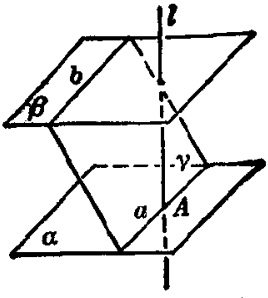
\includegraphics[width=5cm]{../pic/ltjh-ch1-42.png}
        \caption{}\label{fig:ltjh-1-42}
    \end{minipage}
    \qquad
    \begin{minipage}[b]{7cm}
        \centering
        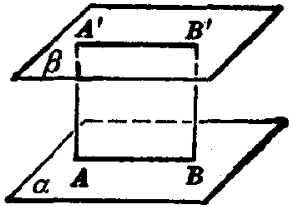
\includegraphics[width=5cm]{../pic/ltjh-ch1-43.png}
        \caption{}\label{fig:ltjh-1-43}
    \end{minipage}
\end{figure}

和两个平行平面同时垂直的直线,叫做这\zhongdian{两个平行平面的公垂线},
它夹在这两个平行平面间的部分,叫做这\zhongdian{两个平行平面的公垂线段}。

如图 \ref{fig:ltjh-1-43}, $\alpha \pingxing \beta$,如果 $AA'$、$BB'$ 都是它们的公垂线段,那么 $AA' \pingxing BB'$。
根据\nameref{dl:lgpmpx-xz}有 $A'B' \pingxing AB$,所以四边形 $ABB'A'$ 是平行四边形, $AA' = BB'$。

由此我们得到,两个平行平面的公垂线段都相等,我们把公垂线段的长度叫做\zhongdian{两个平行平面的距离}。


\begin{lianxi}

\xiaoti{能不能说分别在两个平行平面内的两条直线都平行。}

\xiaoti{下面说法是否正确:}
\begin{xiaoxiaotis}

    \xxt{如果一个平面内的两条直线平行于另一个平面,那么这两个平面平行;}

    \xxt{如果一个平面内的任何一条直线都平行于另一个平面,那么这两个平面平行。}

\end{xiaoxiaotis}

\xiaoti{求证:\zhongdian{夹在两个平行平面间的平行线段相等。}}

\end{lianxi}

